\section{convergenza uniforme}

\begin{definition}[convergenza uniforme]
\mymark{***}
Sia $A$ un insieme non vuoto e
$f\colon A \to \RR$.
Definiamo la \myemph{norma uniforme} (o norma del $\sup$)
di $f$ come
\[
  \Abs{f}_\infty = \sup_{x\in A} \abs{f(x)}
\]

Se anche $g\colon A \to \RR$
definiamo la \emph{distanza uniforme}
\mynote{distanza uniforme}
\index{distanza!uniforme}
tra $f$ e $g$ come
\[
  d_\infty(f,g) = \sup_{x\in A} \abs{f(x)-g(x)}.
\]

Se $f_k$ è una successione di funzioni e $f$ è una funzione, diremo che $f_k$
\emph{converge uniformemente}
\mynote{convergenza uniforme}
\index{convergenza!uniforme}
a $f$
e scriveremo
\[
f_k \To f
\] se
$d_\infty(f_k,f)\to 0$.
\end{definition}


\begin{example}
\label{ex:466533}
La successione
\[
f_k(x) = \sqrt{x^2 + \frac{1}{k}}
\]
converge uniformemente (su tutto $\RR$) alla funzione $f(x) = \abs{x}$. Infatti sia $g_k(x) = f_k(x) - f(x)$. La funzione $g_k$ è derivabile per $x\neq 0$ e per $x>0$ si ha
\[
  g'_k(x) = \frac{x}{\sqrt{x^2+\frac 1 k}} - 1 < 0.
\]
Dunque la funzione $g_k$ è decrescente su $[0,+\infty)$. Per simmetria (è una funzione pari) è crescente su $(-\infty, 0]$. Risulta quindi che il massimo di $g_k$ è in $x=0$. Chiaramente $g_k \ge 0$ quindi si ha:
\[
  \Abs{f_k - f}_\infty = \sup_{x\in \RR} g_k(x) = g_k(0) = \frac{1}{k} \to 0.
\]
Dunque $f_k \To f$.
\end{example}

Osserviamo che in generale $\Abs{f}_\infty$ e $d_\infty(f,g)$ possono assumere il valore $+\infty$ (ad esempio se $A=\RR$, $f(x)=x$ e $g(x)=0$)
e quindi non è detto che siano effettivamente
una norma e una distanza.

\begin{theorem}[proprietà della norma uniforme]
La norma uniforme soddisfa tutte le proprietà di una norma
(Definizione~\ref{def:norma}), salvo il fatto che può assumere valori in $[0,+\infty]$ invece che in $[0,+\infty)$.
\end{theorem}
%
\begin{proof}
Chiaramente la norma uniforme non assume valori negativi in quanto estremo superiore di un insieme (non vuoto) di numeri reali non negativi. Inoltre se $\Abs{f}_\infty=0$ significa che $\abs{f(x)}=0$ per ogni $x$ e dunque $f=0$ (proprietà di separazione).

L'omogenità segue dall'omogeneità del valore assoluto, in quanto si ha
\[
  \sup_{x\in A} \abs{(\lambda \cdot f)(x)}
  = \sup_{x\in A}\abs{\lambda \cdot f(x)}
  = \sup_{x\in A}\abs{\lambda}\cdot \abs{f(x)}
  = \abs{\lambda} \cdot \sup_{x\in A}\abs{f(x)}.
\]

La disuguaglianza triangolare segue dalla disuguaglianza triangolare del valore assoluto, che viene preservata facendone l'estremo superiore:
\[
  \sup_{x\in A} \abs{f(x)+g(x)}
  \le \sup_{x\in A} \Enclose{\abs{f(x)} + \abs{g(x)}}
  \le \sup_{x\in A} \abs{f(x)} + \sup_{x\in A} \abs{g(x)}.
\]
\end{proof}

\begin{theorem}
Sia $A$ un insieme.
Lo spazio vettoriale
delle funzioni limitate $f\colon A \to \RR$
(cioè delle funzioni con norma uniforme finita)
\[
  \B(A) = \{f\in \RR^A\colon \Abs{f}_\infty < +\infty \}
\]
dotato della norma uniforme $\Abs{\cdot}_\infty$ risulta essere uno spazio di Banach (ovvero uno spazio vettoriale normato e completo).
Su tale spazio di Banach la distanza indotta dalla norma è la distanza uniforme $d_\infty$ e la convergenza indotta dalla distanza è la convergenza uniforme.
\end{theorem}
%
\begin{proof}
Per definizione risulta verificato che la norma uniforme $\Abs{\cdot}_\infty$ assume valori finiti su $\B(A)$.
Dunque, in base al teorema precedente, $\Abs{\cdot}_\infty$ è effettivamente una norma e $\B(A)$ risulta quindi essere uno spazio normato. Dimostriamo ora che esso è completo, cioè che le successioni di Cauchy convergono.

Sia $f_k$ una successione di Cauchy in $\B(A)$.
Allora per ogni $x\in A$ risulta che $f_k(x)$ è una successione di Cauchy in $\RR$ in quanto si ha (per definizione di $\sup$)
\[
  \abs{f_k(x) - f_j(x)} \le \Abs{f_k - f_j}_\infty
\]
e quindi se $\Abs{f_k- f_j} < \eps$
a maggior ragione per $x\in A$ fissato si ha $\abs{f_k(x)-f_j(x)} < \eps$.

Dunque per ogni $x\in A$ la successione numerica $f_k(x)$ converge in quanto $\RR$ è completo. Posto $f(x) = \lim f_k(x)$ abbiamo dunque trovato un candidato limite della successione.
Dovremo ora mostrare che $f\in \B(A)$ e che $f_k$ converge uniformemente a $f$.
Per ogni $\eps>0$ per la condizione di Cauchy dovrà esistere $N\in \NN$ tale che se $k,j>N$ allora
\[
  d_\infty(f_k,f_j) < \eps.
\]
Ma allora per ogni $x\in A$, per ogni $k>N$ e per ogni $j>N$ si avrà:
\[
  \abs{f_k(x) - f(x)} \le \abs{f_k(x) - f_j(x)} +
  \abs{f_j(x) - f(x)} < \eps + \abs{f_j(x)-f(x)}.
\]
Visto che per ogni $x$ si ha $f_j(x) \to f(x)$, per ogni $x$ esiste un $j$ tale che $\abs{f_j(x)-f(x)} < \eps$ e quindi possiamo concludere che
\[
  \abs{f_k(x)-f(x)} < 2\eps.
\]
Facendo il $\sup$ per $x\in A$ si ottiene dunque
\[
  \Abs{f_k -f}_\infty \le 2 \eps.
\]
Abbiamo quindi verificato la definizione di limite $\Abs{f_k -f}_\infty\to 0$. In particolare $\Abs{f}_\infty < +\infty$ in quanto vale la disuguaglianza triangolare
\[
  \Abs{f}_\infty \le \Abs{f-f_k}_\infty + \Abs{f_k}_\infty < +\infty
\]
essendo $\Abs{f-f_k}_\infty \to 0$ e $\Abs{f_k}_\infty < +\infty$.
\end{proof}

\begin{definition}[convergenza puntuale]
\mymark{***}
Sia $f_k\colon A \to \RR$ una successione di funzioni
e sia $f\colon A \to \RR$ una funzione.
Se per ogni $x\in A$ si ha $f_k(x)\to f(x)$ diremo che
la successione $f_k$
\emph{converge puntualmente}
\mynote{convergenza puntuale}
\index{convergenza!puntuale}
ad $f$.
\end{definition}

\begin{theorem}[convergenza uniforme implica convergenza puntuale]
\mymark{***}
Sia $f_k\colon A \to \RR$ una successione di funzioni.
Se $f_k$ converge uniformemente ad una funzione $f$ allora $f_k$ converge puntualmente ad $f$.
\end{theorem}
%
\begin{proof}
E' sufficiente osservare che per ogni $x\in A$ si ha
\[
  \abs{f_k(x)-f(x)} \le \sup_{y\in A} \abs{f_k(y)-f(y)}
   = \Abs{f_k-f}_\infty \to 0.
\]
\end{proof}

\begin{example}[successione che converge puntualmente ma non uniformemente]
\mymark{***}
Sia $f_k\colon [0,1]\to \RR$ la successione di funzioni definita da $f_k(x)=x^k$. Se $x\in[0,1)$ si ha $x^k \to 0$ mentre se $x=1$ si ha $x^k \to 1$. Dunque la successione $f_k$ converge puntualmente alla funzione
\[
f(x) =
 \begin{cases}
  0 & \text{se $x\in [0,1)$}\\
  1 & \text{se $x=1$}.
 \end{cases}
\]
Osserviamo però che
\[
  d_\infty(f_k,f) = \sup_{x\in [0,1]} \abs{f_k(x)-f(x)}
  \ge \lim_{x\to 1^-} \abs{f_k(x) - f(x)} = 1.
\]
dunque non ci può essere convergenza uniforme di $f_k$ verso $f$.
\end{example}

E' facile convincersi che la successione $f_k$ dell'esempio precedente, oltre a non convergere uniformemente non ammette nessuna estratta convergente uniformemente. Perciò tale successione non può essere contenuta in nessun compatto di $C^0([0,1])$. In particolare il disco unitario
\[
  D = \{f\in C^0([0,1])\colon \Abs{f}_\infty \le 1\}
\]
risulta essere un insieme chiuso e limitato che però non è compatto.

\begin{theorem}[continuità del limite uniforme]
\mymark{***}
Sia $X$ uno spazio metrico e siano $f_k\colon X\to \RR$
funzioni continue che
convergono uniformemente ad una funzione $f\colon X \to \RR$. Allora anche $f$ è continua.
\end{theorem}
%
\begin{proof}
\mymark{***}
Fissato $x_0\in X$ basta dimostrare che per ogni $\eps>0$
esiste $\delta>0$ tale che se $d(x,x_0)< \delta$ allora $\abs{f(x)-f(x_0)} < 3 \eps$.
Per definizione di convergenza uniforme dato $\eps>0$
esiste un $N\in \NN$ (in realtà ne esistono infiniti) per cui
$d_\infty(f_N,f)< \eps$. Per la continuità di $f_N$ in corrispondenza dello stesso $\eps$ esiste $\delta>0$
tale che se $d(x,x_0) < \delta$ allora $\abs{f_N(x)-f_N(x_0)} < \eps$. Ma allora se $d(x,x_0)<\delta$ si ha
\begin{align*}
\abs{f(x)-f(x_0)}
&\le \abs{f(x) - f_N(x)}
 + \abs{f_N(x)-f_N(x_0)}
 + \abs{f_N(x_0) - f(x_0)} \\
 &\le \Abs{f-f_N}_\infty + \eps + \Abs{f-f_N}_\infty
  \le 3\eps.
\end{align*}
\end{proof}

\begin{theorem}[completezza di $C^0({[a,b]})$]
\mymark{***}
\mynote{$C^0([a,b])$ è completo}
\index{completezza!di $C^0([a,b])$}
Lo spazio $C^0([a,b])$ delle funzioni continue definite su un intervallo chiuso e limitato, dotato della norma uniforme $\Abs{\cdot}_\infty$ risulta essere uno spazio di Banach (ovvero uno spazio vettoriale normato e completo).
\end{theorem}
%
\begin{proof}
Per il teorema di Weierstrass ogni funzione continua definita sul compatto $[a,b]$ è limitata. Dunque $C^0([a,b])$ è un sottospazio vettoriale di $\B([a,b])$. Inoltre il teorema precedente (continuità del limite) ci dice che $C^0([a,b])$ è un sottospazio chiuso di $\B([a,b])$.
Ma $\B([a,b])$ è completo e quindi anche $C^0([a,b])$ essendo chiuso in $\B([a,b])$ è completo.
\end{proof}

La norma uniforme è la norma naturale su $C^0([a,b])$ in quanto lo rende uno spazio completo. Per questo motivo la norma uniforme sulle funzioni continue
viene anche chiamata \emph{norma $C^0$} e si
può denotare nel modo seguente:
\index{$\Abs{\cdot}_{C^0}$}
\index{norma!$C^0$}
\[
  \Abs{f}_{C^0} = \Abs{f}_{C^0([a,b])} = \Abs{f}_\infty
  \qquad\text{per $f\in C^0([a,b])$.}
\]

\section{limite uniforme di derivate e integrali}

\begin{theorem}[scambio del limite con l'integrale]
\mymark{***}
Siano $a,b\in \RR$, $a\le b$.
Siano $f_k\in C^0([a,b])$ funzioni che convergono uniformemente
ad una funzione $f\in C^0([a,b])$.
Allora
\[
  \lim_{k\to+\infty}\enclose{\int_a^b f_k(x)\, dx}
  = \int_a^b f(x)\, dx
  = \int_a^b \enclose{\lim_{k\to +\infty} f_k(x)} \, dx.
\]

Inoltre scelto qualunque $x_0\in [a,b]$ e posto
\[
  F_k(x) = \int_{x_0}^x f_k(t)\, dt,
  \qquad
  F(x) = \int_{x_0}^x f(t)\, dt
\]
si ha che $F_k$ converge uniformemente a $F$.
\end{theorem}
%
\begin{proof}
\mymark{***}
Banalmente si ha
\begin{align*}
  \abs{\int_a^b f_k(x)\, dx - \int_a^b f(x)\, dx}
  &\le \int_a^b \abs{f_k(x) - f(x)}\, dx \\
  &\le \int_a^b \Abs{f_k - f}_\infty\, dx \\
  &= (b-a) \Abs{f_k -f}_\infty
  \to 0.
\end{align*}

Se poi definiamo $F$ e $F_k$ come nell'enunciato, si ha
\begin{align*}
  \Abs{F_k-F}
  &= \sup_{x\in [a,b]} \abs{\int_c^x f_k(t)-f(t)\, dt} \\
  &\le \sup_{x\in [a,b]} \abs{x-c} \cdot \Abs{f_k-f}_\infty \\
  &\le (b-a) \cdot \Abs{f_k-f}_\infty
  \to 0.
\end{align*}
\end{proof}

Il teorema precedente è equivalente a dire che l'operatore integrale $S\colon C^0([a,b]) \to C^0([a,b])$
\[
S(f)(x) = \int_{x_0}^x f(t)\, dt
\]
che fissato $x_0 \in [a,b]$ associa ad una funzione $f\in C^0([a,b])$ la sua funzione integrale, è un operatore continuo rispetto alla norma uniforme.

In realtà le ipotesi per garantire la possibilità di scambiare
il limite con l'integrale sono molto più deboli, per avere un teorema
con ipotesi ottimali sarebbe però necessario introdurre l'integrale di Lebesgue,
cosa che non vogliamo fare in questo corso. Un enunciato più generale
che possiamo dimostrare facilmente con gli strumenti
a nostra disposizione è il seguente.

\begin{theorem}[convergenza dominata quasi uniforme]
\label{th:convergenza_dominata}%
\mymargin{convergenza dominata}%
\index{teorema!di convergenza dominata}%
Siano $f_k\colon [a,b) \to \RR$, funzioni continue
sull'intervallo $[a,b)$ con $a\in \RR$, $b\in (a,+\infty]$
e supponiamo che esista $g\colon [a,b)\to \RR$
integrabile in senso improprio su $[a,b)$ con integrale finito e tale
che
\[
\abs{f_k(x)}\le g(x)
\]
per ogni $k\in \NN$ e ogni $x\in [a,b)$.

Supponiamo inoltre che per
ogni $x\in[a,b)$ esista e sia finito il limite
\[
  f(x) = \lim_{k\to +\infty} f_k(x)
\]
e che per ogni $\beta<b$ la successione $f_k$ converga uniformemente
ad $f$ sull'intervallo $[a,\beta]$.

Allora $f_k$ ed $f$ sono integrabili in senso improprio su $[a,b)$ e si ha
\[
  \lim_{k\to+\infty} \int_a^b f_k(x)\, dx = \int_a^b f(x)\, dx.
\]

Ovviamente, per simmetria, vale un risultato analogo per funzioni definite su intervalli
aperti a sinistra $(a,b]$ e su unioni finite di tali intervalli.
\end{theorem}
%
\begin{proof}
Ogni $f_k$ è assolutamente integrabile in senso improprio in quanto
$\abs{f_k}\le g$ dove $g$ ha integrale finito per ipotesi.
Visto che $f_k$ converge uniformemente a $f$ su ogni intervallo $[a,\beta]$
la funzione $f$ è anch'essa continua su ogni $[a,\beta]\subset[a,b)$
e quindi è continua su tutto $[a,b)$. Inoltre passando al limite (puntuale)
nella stima $\abs{f_k(x)}\le g(x)$ si trova che vale anche $\abs{f(x)}\le g(x)$
e quindi anche $f$ è integrabile su $[a,b)$ con integrale finito.

Su ogni $[a,\beta]\subset [a,b)$ possiamo applicare il teorema precedente
in quanto abbiamo convergenza uniforme:
\[
  \lim_{k\to+\infty} \int_a^\beta f_k(x)\, dx = \int_a^\beta f(x)\, dx.
\]
razie alla continuità della funzione integrale,
per ogni $\eps>0$ esiste $\beta<b$ per cui risulta
\[
  \int_{\beta}^b g(x)\, dx < \eps.
\]
Allora si ha
\begin{equation}\label{eq:438948}
\begin{aligned}
  \abs{\int_a^b f_k(x)\, dx - \int_a^b f(x)\, dx}
  &= \abs{\int_a^\beta f_k(x)\, dx - \int_a^\beta f(x)\, dx}\\
  &\quad + \abs{\int_\beta^b (f_k(x) - f(x))\, dx }.
   \end{aligned}
\end{equation}
Il primo addendo tende a zero per $k\to +\infty$ in quanto
sull'intervallo $[a,\beta]$ c'è convergenza uniforme di $f_k$
a $f$ e quindi possiamo applicare il teorema precedente
di scambio del limite con l'integrale. Per il secondo addendo
si ha invece
\begin{align*}
\abs{\int_\beta^b (f_k(x) - f(x))\, dx }
&\le \int_\beta^b \abs{f_k(x)-f(x)}\, dx\\
&\le \int_\beta^b \abs{f_k(x)}\, dx + \int_\beta^b \abs{f(x)}\, dx\\
&\le 2 \int_\beta^b g(x)\, dx \le \eps.
\end{align*}
Dunque per ogni $\eps>0$ esiste $\beta<b$ tale che per $k$ abbastanza
grande
la quantità in~\eqref{eq:438948} risulta essere inferiore a $2\eps$.
Abbiamo quindi verficato la tesi tramite la definizione di limite.
\end{proof}

\begin{example}
La successione $f_k(x) = \sin(x^k)$ converge puntualmente a $f(x)=0$ sull'intervallo
$\left[0,\frac \pi2\right)$ e la convergenza è uniforme su ogni intervallo $[0,\beta]$
con $\beta < \frac \pi 2$ (verificare!).
Inoltre $\abs{f_k(x)} = \sin(x^k) \le 1$ per ogni $x\in \Enclose{0,\frac \pi 2}$
e $\int_0^{\frac \pi 2} 1\, dx = \frac \pi 2 < +\infty$.
Dunque possiamo applicare il teorema di convergenza dominata e,
scambiando il limite con l'integrale possiamo dedurre che
\[
  \int_0^{\frac \pi 2} \sin (x^k)\, dx \to 0, \qquad \text{per $k\to +\infty$.}
\]

\end{example}

\begin{theorem}[scambio del limite con la derivata]
\mymark{***}
Sia $I\subset \RR$ un intervallo e siano $f_k\in C^1(I)$ funzioni tali che $f_k(x_0)$ converge per almeno un punto $x_0\in I$ e la successione delle derivate $f_k'$ converge
ad una funzione $g\colon I \to \RR$
uniformemente su ogni intervallo chiuso e limitato $[a,b]\subset I$. Allora esiste $f\in C^1(I)$ tale che $f'=g$ e $f_k$ converge a $f$ uniformemente su ogni intervallo chiuso e limitato $[a,b]\subset I$.
In queste ipotesi si può quindi scambiare la derivata con il limite:
\[
  \lim_{k\to +\infty}\enclose{\frac{d}{dx} f_k(x)}
  = f'(x)
  = \frac{d}{dx} \enclose{\lim_{k\to +\infty} f_k(x)},
  \qquad \forall x \in I.
\]
\end{theorem}
%
\begin{proof}
\mymark{***}
Per ipotesi esiste $y_0\in \RR$ tale che $f_k(x_0) \to y_0$.
Definiamo
\[
  f(x) = y_0 + \int_{x_0}^x g(t)\, dt.
\]
Per la continuità del limite uniforme sappiamo che $g$ è continua, dunque possiamo applicare il teorema fondamentale del calcolo per dedurre che $f'=g$. Mostriamo ora che su ogni intervallo $[a,b]\subset I$ si ha $f_k \To f$. Per la formula fondamentale del calcolo integrale si ha:
\[
  \int_{x_0}^x f_k'(t) dt = f_k(x) - f_k(x_0)
\]
dunque
\begin{align*}
  \sup_{x\in [a,b]}\abs{f_k(x) - f(x)}
  &= \sup_{x\in [a,b]} \abs{f_k(x_0) + \int_{x_0}^x f_k'(t) - y_0 - \int_{x_0}^x g(t)\, dt} \\
  &\le \abs{f_k(x_0) - y_0} + \sup_{x\in [a,b]}\abs{\int_{x_0}^x \abs{f_k'(t) - g(t)}\, dt} \\
  &\le \abs{f_k(x_0) - y_0} + (b-a)\Abs{f_k' - g} \to 0.
\end{align*}
\end{proof}

Lo spazio $C^1([a,b])$ è un sottospazio vettoriale di $C^0([a,b])$ ma non è chiuso, come si deduce dall'esempio~\ref{ex:466533} (si potrebbe anzi dimostrare che $C^1$ è denso in $C^0$) dunque $C^1$ non è completo rispetto alla norma uniforme.
Per trasformare lo spazio $C^1([a,b])$ in uno spazio di Banach
possiamo definire una norma più forte, come ad esempio
questa:
\[
  \Abs{f}_{C^1} = \Abs{f}_\infty + \Abs{f'}_\infty.
\]
\begin{theorem}[$C^1$ spazio di Banach]
\mymark{*}
Lo spazio vettoriale $C^1([a,b])$ dotato della norma $\Abs{\cdot}_{C^1}$ risulta essere uno spazio di Banach.
\end{theorem}
%
\begin{proof}
E' facile verificare che $\Abs{\cdot}_{C^1}$ è una norma su $C^1([a,b])$, dobbiamo solo verificare che lo spazio risulta completo. Sia dunque $f_k$ una successione di Cauchy rispetto alla norma $C^1$. Allora $f_k'$ e $f_k$ sono entrambe successioni di Cauchy in $C^0$ in quanto $\Abs{f_k}_\infty \le \Abs{f_k}_{C^1}$ e $\Abs{f_k'}_\infty \le \Abs{f_k}_{C^1}$.
Dunque, per la completezza di $C^0$, sappiamo che esistono $f,g\in C^0([a,b])$ tali che $f_k\To f$ e $f_k'\To g$.
In base al teorema di scambio del limite con la derivata possiamo affermare che $f\in C^1$ e $f'=g$, dunque
\[
  \Abs{f_k-f}_{C^1} = \Abs{f_k-f}_\infty + \Abs{f_k'-g}_\infty \to 0.
\]
\end{proof}

Il teorema di scambio del limite con l'integrale ci dice che
l'operatore integrale $S\colon C^0 \to C^1$ è continuo tra i due spazi di Banach. Anche l'operatore differenziale $D\colon C^1 \to C^0$ $f\mapsto Df = f'$ è ovviamente continuo.

\section{serie di funzioni}

Se $f_k\colon A \to \RR$ è una successione di funzioni
definite su uno stesso insieme $A$, possiamo considerare (come abbiamo già fatto per le successioni numeriche) la successione delle somme parziali:
\[
  S_n(x) = \sum_{k=0}^n f_k(x), \qquad x\in A.
\]
Tale successione si chiama \emph{serie} corrispondente alla successione di funzioni $f_k$
e si indica a volte come $\sum f_n$. Per ogni $x$ in cui la serie è convergente si può quindi definire la
\myemph{somma} della serie
\[
  S(x) = \sum_{k=0}^{+\infty} f_k(x) = \lim_{n\to +\infty} S_n(x).
\]
La somma $S$ è dunque il limite puntuale della successione delle somme parziali $S_n$.

I teoremi che abbiamo dimostrato per le successioni di funzioni sono quindi validi anche per le serie di funzioni. Basterà ricordare che la \emph{convergenza uniforme della serie}
\mynote{convergenza uniforme di una serie}%
\index{serie!convergenza uniforme}%
\index{convergenza!uniforme di una serie}%
 è la convergenza uniforme delle somme parziali. Dunque $\sum f_k$ converge uniformemente a $S$ se $S_n \To S$ ovvero se
\[
  \Abs{S - S_n}_\infty = \Abs{\sum_{k=n+1}^{+\infty} f_k}_\infty \to 0
  \qquad \text{per $n\to +\infty$.}
\]



\begin{theorem}[integrale di una serie di funzioni]
\label{th:integrale_serie}
\mymark{**}%
\index{teorema!integrazione di una serie di funzioni}%
\index{serie!integrale}%
\mynote{integrazione di una serie}%
Sia $f_k\colon [a,b]\to\RR$ una successione di funzioni continue definite sull'intervallo $[a,b]\subset \RR$.
Se la serie $\sum f_k$ converge uniformemente
allora si può scambiare l'integrale con la somma della serie:
\[
  \int_a^b \enclose{\sum_{k=0}^{+\infty} f_k(t)}\, dt
  = \sum_{k=0}^{+\infty} \enclose{\int_a^b f_k(t)\, dt}
  \qquad \forall x \in I.
\]
\end{theorem}
\begin{proof}
\mymark{**}
La dimostrazione è una semplice conseguenza del fatto che lo scambio può essere fatto sulle somme finite e il passaggio al limite può essere fatto grazie al teorema di scambio del limite con l'integrale.

Sia $S_n = \sum f_n$ la successione delle somme parziali e sia $S$ il limite delle somme parziali. Per ipotesi $S_n\To S$. Applicando il teorema di scambio dell'integrale con il limite si ha
\[
  \lim_{n\to +\infty} \int_a^b S_n(t)\, dt = \int_a^b S(t)\, dt.
\]
Ma da un lato, sfruttando l'additività dell'integrale sulle somme finite:
\begin{align*}
  \lim_{n\to +\infty} \int_a^b S_n(t)\, dt
   &= \lim_{n\to+\infty}\int_a^b \enclose{\sum_{k=0}^n f_k(t)} \,  dt\\
   &= \lim_{n\to+\infty}\sum_{k=0}^n \enclose{\int_a^b f_k(t)\, dt}\\
   &= \sum_{k=0}^\infty \enclose{\int_a^b f_k(t)\, dt}
\end{align*}
e dall'altro lato:
\[
  \int_a^b S(t)\, dt = \int_a^b \enclose{\sum_{k=0}^{+\infty} f_k(t)}\, dt.
\]
\end{proof}

\begin{theorem}[derivata di una serie di funzioni]
\mymark{**}
\index{teorema!derivazione di una serie di funzioni}
\index{serie!derivata}
\mynote{derivazione di una serie}
Sia $f_k\colon I\to\RR$ una successione di funzioni continue definite sull'intervallo $I$. Se le funzioni $f_k$ sono di classe $C^1$ e la serie delle derivate $\sum f_k'$ converge uniformemente
su ogni intervallo chiuso e limitato $[a,b]\subset I$
e se c'è almeno un punto $x_0\in I$ tale che la serie
$\sum f_k(x_0)$ converge, allora
\[
  \frac{d}{dx} \sum_{k=0}^{+\infty} f_k(x) = \sum_{k=0}^{+\infty} \frac{d}{dx}f_k(x)
  \qquad \forall x \in I.
\]
\end{theorem}

\begin{proof}
\mymark{**}
Sia $S_n$ la successione delle somme parziali. Per ipotesi sappiamo che esiste una funzione $T\colon I \to \RR$ tale che $S_n' \To T$ in ogni intervallo $[a,b]\subset I$.
Sappiamo inoltre che $S_n(x_0)$ converge.
Dunque possiamo applicare il teorema di scambio del limite con la derivata per ottenere che esiste $S\in C^1(I)$ tale che
 $S_n(x)\to S(x)$ per ogni $x\in I$ e
\[
   S'(x) = T(x) \qquad \forall x\in I.
\]
Ma da un lato
\begin{align*}
S'(x)
&= \frac{d}{dx} \lim_{n\to +\infty} S_n(x) \\
&= \frac{d}{dx} \sum_{k=0}^{+\infty} f_k(x)
\end{align*}
e dall'altro lato
\begin{align*}
T(x)
&= \lim_{n\to +\infty} S_n'(x)
 = \lim_{n\to +\infty} \frac{d}{dx} \sum_{k=0}^n f_k(x) \\
&= \lim_{n\to +\infty} \sum_{k=0}^n f_k'(x)
 = \sum_{k=0}^{+\infty} f_k'(x).
\end{align*}
\end{proof}

La convergenza uniforme di una serie non è molto semplice da verificare. Più semplice è la seguente condizione, che vedremo essere più forte.

\begin{definition}[convergenza totale di una serie di funzioni]
\mymark{***}
Siano $f_k\colon A \to \RR$ funzioni definite su un insieme $A\subset \RR$. Diremo che la serie di funzioni $\sum f_k$
\emph{converge totalmente}
\mynote{convergenza totale}
\index{convergenza!totale}
se la serie numerica $\sum \Abs{f_k}_\infty$
è convergente.
\end{definition}

\begin{theorem}[convergenza totale]
\mymark{***}
Se la serie $\sum f_n$ converge totalmente allora converge uniformemente.
\end{theorem}
%
\begin{proof}
\mymark{***}
A $x$ fissato
la serie $\sum f_n(x)$ converge assolutamente in quanto
\[
  \sum_{k=0}^\infty \abs{f_n(x)}
  \le \sum_{k=0}^\infty \Abs{f_n}_\infty < +\infty.
\]
Dunque la serie converge e posto
\[
  S_n(x) = \sum_{k=0}^n f_k(x), \qquad
  S(x) = \sum_{k=0}^{+\infty} f_k(x)
\]
si ha che $S_n\to S$ puntualmente.
Per mostrare che $S_n \To S$ basta osservare che per
$n\to +\infty$ si ha:
\[
  \abs{S(x) - S_n(x)}
  = \abs{\sum_{k=n+1}^{+\infty} f_k(x)}
  \le \sum_{k=n+1}^{+\infty}\abs{f_k(x)}
  \le \sum_{k=n+1}^{+\infty}\Abs{f_k}_\infty \to 0.
\]
\end{proof}

\begin{theorem}[convergenza totale delle serie di potenze]
\label{th:convergenza_totale}
\mymark{***}%
Sia $\sum a_n z^n$ una serie di potenze e sia $R\in[0,+\infty]$ il suo raggio di convergenza. Allora la serie converge totalmente su ogni disco $D_r$ con $r<R$.
\end{theorem}
%
\begin{proof}
Ora osserviamo che sul disco di raggio $r$ si ha $\Abs{a_k z^k}_\infty = \abs{a_k} r^k$ e dunque
\[
\sum_{k=0}^{+\infty} \Abs{a_k z_k}_\infty
= \sum_{k=0}^{+\infty} \abs{a_k}r^k < +\infty
\]
in quanto la serie $\sum a_k z^k$ converge assolutamente per $z=r$ essendo $r<R$.
\end{proof}

\begin{corollary}
\label{cor:derivata_serie_potenze}
\mymark{**}
La serie di potenze
\[
  f(x) = \sum_{k=0}^{+\infty} a_k x^k
\]
ha lo stesso raggio di convergenza $R$ della serie delle derivate
\[
  g(x) = \sum_{k=1}^{+\infty} k a_k x^{k-1}
\]
e per $x\in (-R,R)$ si ha
\[
  f'(x) = g(x).
\]
\end{corollary}
%
\begin{proof}
Che le due serie abbiano lo stesso raggio di convergenza l'abbiamo già dimostrato nel Teorema~\ref{th:raggio_serie_derivate}. Nel teorema precedente abbiamo mostrato che su ogni intervallo $[-r,r]$ con $r<R$ la serie di potenze con somma $f$ converge totalmente. Dunque converge uniformemente e possiamo scambiare la derivata con la somma per ottenere $f'(x) = g(x)$.
\end{proof}

\begin{example}
Sappiamo che la serie di potenze
\[
f(x) = \sum_{k=1}^{+\infty} \frac{x^k}{k}
\]
ha raggio di convergenza $R=1$ (si usi ad esempio il criterio del rapporto). La serie delle derivate è
\[
 g(x) = \sum_{k=1}^{+\infty} x^{k-1} = \sum_{k=0}^{+\infty}x^k = \frac{1}{1-x}.
\]
Dunque per $\abs{x}<1$ si ha
\[
  f'(x) = g(x) = \frac{1}{1-x}
\]
da cui
\[
 f(x) = f(0) + \int_0^x f'(t)\, dt = \int_0^x \frac{1}{1-t}\, dt
  = \Enclose{-\ln(1-t)}_0^x = -\ln(1-x).
\]
Abbiamo quindi scoperto che vale
\[
  \sum_{k=1}^{+\infty} \frac{x^k}{k} = - \ln (1-x) \qquad\text{per ogni $x\in (-1,1)$.}
\]
Osserviamo ora che la serie con somma $f(x)$
non converge per $x=1$ (serie armonica) ma
converge per $x=-1$ (criterio di Leibniz).
Per il Teorema~\ref{th:lemma_abel} (lemma di Abel)
sappiamo che la funzione $f(x)$ è continua nel punto $x=-1$ e dunque possiamo concludere che
\[
  \sum_{k=1}^{+\infty} \frac{x^k}{k} = -\ln(1-x)
  \qquad \forall x \in [-1,1).
\]
In particolare abbiamo trovato la somma della serie armonica a serie alterni:
\[
  \sum_{k=1}^{+\infty} \frac{(-1)^{k+1}}{k} = - f(x) = \ln 2.
\]

Osserviamo che queste informazioni sono coerenti con lo sviluppo di Taylor di $\ln(1+x)$ che avevamo già determinato. Ma non sono conseguenza di esso, in quanto lo sviluppo di Taylor ci dà informazioni solamente per $x\to 0$ mentre ora abbiamo ottenuto informazioni per ogni $x$ in $[-1,1)$.
 \end{example}

\begin{example}
Applichiamo l'idea precedente alla funzione $\arctg$. Si ha
\[
  \arctg'(x) = \frac{1}{1+x^2} = \sum_{k=0}^{+\infty} (-x^2)^k
  = \sum_{k=0}^{+\infty} (-1)^k x^{2k}
  = \sum_{k=0}^{+\infty} \frac{(-1)^k}{2k+1}(x^{2k+1})'.
\]
La serie
\[
 f(x) = \sum_{k=0}^{+\infty}\frac{(-1)^k}{2k+1} x^{2k+1}
\]
ha raggio di convergenza $R=1$ e dunque per ogni $x\in(-1,1)$ sappiamo che la serie delle derivate converge alla derivata della serie da cui
\[
  f'(x) = \arctg' x.
\]
Visto che $f(0) = 0 = \arctg 0$ possiamo concludere che $f(x) =\arctg x$ per ogni $x\in (-1,1)$.
La serie è convergente anche per $x=1$, per il criterio di Leibniz. Per continuità (Lemma di Abel) si ottiene che $f(1) = \arctg 1$. Dunque
\[
  \arctg x = \sum_{k=0}^{+\infty}\frac{(-1)^k}{2k+1}x^{2k}
  \qquad \forall x \in (-1,1].
\]
In particolare per $x=1$ si ottiene la formula di \myemph{Gregory-Leibniz}
\index{$\pi$!formula di Gregory-Leibniz}
\index{Gregory!approssimazione $\pi$}
\index{Leibniz!approssimazione $\pi$}
\index{formula!di Gregory-Lebniz per $\pi/4$}
\[
  \frac{\pi}{4} = \sum_{k=0}^{+\infty} \frac{(-1)^k}{2k+1} =
   1 - \frac{1}{3} + \frac{1}{5} - \frac{1}{7} + \dots
\]
\end{example}

\section{divagazione sui frattali autosimili}

\begin{definition}
Siano $A$ e $B$ sottoinsiemi non vuoti di $\RR^n$.
Definiamo la \emph{distanza di Hausdorff}
\mynote{distanza di Hausdorff}
\index{distanza!di Hausdorff}
tra $A$ e $B$ come:
\[
  d_{\H}(A,B) = \max\big\{\sup_{a\in A}\inf_{b\in B} \abs{a-b}, \sup_{b\in B} \inf_{a\in A} \abs{a-b}\big\}.
\]

Definiamo
\[
 \K(\RR^n) = \{A \subset \RR^n \colon \text{$A$ chiuso, limitato, non vuoto}\}.
\]
\end{definition}

\begin{theorem}[caratterizzazione della distanza di Hausdorff]
Se $A$ e $B$ sono compatti di $\RR^n$ (cioè chiusi e limitati) allora
per ogni $r \in \RR$
si ha
\[
  d_\H(A,B) \le r
\]
se e solo se valgono entrambe le seguenti proprietà:
\begin{enumerate}
\item per ogni $a\in A$ esiste $b\in B$ tale che $\abs{a-b}\le r$;
\item per ogni $b\in B$ esiste $a\in A$ tale che $\abs{a-b}\le r$.
\end{enumerate}
\end{theorem}
%
\begin{proof}
Per ogni compatto non vuoto $A$ e per ogni $x\in \RR^n$ definiamo
la distanza tra il punto $x$ e l'insieme $A$ come:
\[
  d(x,A) = \min_{a\in A} \abs{x-a}.
\]
Il minimo esiste in quanto $A$ è compatto e $a\mapsto d(x,a)$ è una funzione continua. Fissato $A$ la funzione $x\mapsto d(x,A)$ è anch'essa continua, anzi è $1$-lipschitziana. Infatti se $x'\in \RR^n$ esiste $a'\in A$ tale che $d(x',A) = d(x',a')$ e dunque
\[
  d(x,A) = \min_{x\in A} \abs{x-a} \le \abs{x-a'} \le \abs{x-x'} + \abs{x'- a'}
   = \abs{x-x'} + d(x',A)
\]
da cui $d(x,A) - d(x',A)\le \abs{x-x'}$.
Scambiando $x$ e $x'$ si ottiene anche la disuguaglianza inversa da cui la $1$-lipschitzianità di $d(x,A)$. Dunque sui compatti la funzione $d(x,A)$ assume sempre massimo e si ha:
\[
d_\H(A,B) = \max\{\max_{a_\in A} d(a,B), \max_{b\in B} d(b,A)\}.
\]

In particolare se $d_\H(A,B) \le r$ per ogni $a\in A$ si deve avere $d(a,B) \le r$ e per ogni $b\in B$ si deve avere $d(b,A) \le r$. Ma allora valgono le due proprietà dell'enunciato.

Viceversa se vale la proprietà 1.\ allora $d(a,B)\le r$ e se vale la 2.\ $d(b,A)\le r$ e di conseguenza $D_\H(A,B) \le r$.
\end{proof}

\begin{theorem}[distanza di Hausdorff]
La distanza di Hausdorff $d_\H$ è una distanza su $\K(\RR^n)$ e lo spazio metrico $\K(\RR^n)$ è completo.
\end{theorem}
%
\begin{proof}
Chiaramente se $A,B$ sono non vuoti si ha $d_\H(A,B) \ge 0$.
Inoltre, in base alla caratterizzazione del teorema precedente è facile osservare che $d_\H(A,B) < +\infty$.

Se $d_\H(A,B) = 0$ significa che per ogni $a\in A$ esiste $b\in B$ tale che $\abs{a-b}=0$. Cioè $b=a$. Dunque $A\subset B$. Scambiando i ruoli di $A$ e $B$ si ottiene anche $B\subset A$ da cui $A=B$.

Che sia $d_\H(A,B) = d_\H(B,A)$ è ovvio in quanto la definizione è simmetrica in $A$ e $B$.

Verifichiamo ora la disuguaglianza triangolare. Siano $A,B,C$ tre compatti non vuoti. Per ogni $a\in A$ esiste $b\in B$ tale che $\abs{a-b} \le d_\H(A,B)$ e per tale $b \in B$ esiste un $c\in C$ tale che $\abs{b-c} \le d_\H(B,C)$. Dunque per ogni $a\in A$ esiste un $c\in C$ tale che
\[
  \abs{a-c} \le \abs{a-b} + \abs{b-c} \le d_\H(A,B) + d_\H(B,C).
\]
Scambiando i ruoli di $A$ e $C$ si ottiene anche la condizione simmetrica e dunque, per la caratterizzazione della distanza di Hausdorff si ottiene la disuguaglianza triangolare:
\[
  d_\H(A,C) \le d_\H(A,B) + d_\H(B,C).
\]

Abbiamo quindi verificato che $d_\H$ è una distanza su $\K(\RR^n)$. Verifichiamo ora che $\K(\RR^n)$ è completo.

Sia $A_k\in\K(\RR^n)$ una successione di Cauchy.
Senza perdita di generalità possiamo supporre che
\[
  d_\H(A_k,A_{k+1}) \le \frac{1}{2^k}.
\]
Infatti essendo $A_k$ di Cauchy è possibile trovarne una sottosuccessione con tale proprietà, e se poi dimostriamo che la sottosuccessione converge allora l'intera successione, essendo di Cauchy, deve convergere.

Consideriamo come candidato limite l'insieme di tutti i possibili limiti di punti degli insiemi $A_k$:
\[
  A = \{x\in \RR^n
  \colon \exists x_k \in A_k\colon x_k \to x\}.
\]

Per prima cosa vogliamo verificare che $A$ non è vuoto. Scelto un punto qualunque $a_0 \in A_0$ esiste $a_1 \in A_1$ tale che $\abs{a_0 - a_1} = d_\H(A_0,A_1)$. Iterando otteniamo una successione di punti $a_k \in A_k$ tale che $\abs{a_k - a_{k+1}} \le d_\H(A_k,A_{k+1}) \le 1/2^k$.
Dunque $a_k$ è una successione di Cauchy in $\RR^n$ ed essendo $\RR^n$ completo dovrà convergere ad un punto $a$ che quindi è un punto di $A$.

Avendo assunto $d_\H(A_k, A_{k+1}) < 1/2^k$ si ottiene (sommando la serie geometrica):
\[
 d_\H(A_k, A_n) \le \sum_{j=k}^{n-1} d_\H(A_j, A_{j+1}) \le \frac{2}{2^k}\qquad \text{se $n>k$}.
\]
Questo ci permette di dimostrare che per ogni $a\in A$ e per ogni $k\in \NN$ esiste $a_k \in A_k$ tale che
$\abs{a - a_k}\le 4/2^k$. Infatti se a distanza $4/2^k$ non ci fossero punti di $A_k$ allora a distanza $2/2^k$ non ci potrebbero essere punti di $A_n$ per nessun $n>k$ in quanto visto che $d_\H(A_k,A_n) \le 2/2^k$ se ci fosse un punto di $A_n$ a distanza inferiore a $2/2^k$ ci dovrebbe anche essere un punto di $A_k$ a distanza inferiore a $4/2^k$. Ma questo è impossibile perché per come è definito $A$ deve esistere $x_n \in A_n$ tale che $x_n \to a$. Abbiamo quindi mostrato che
\[
  \sup_{a\in A} \inf_{b\in A_k} \abs{a-b} \le 4/2^k \to 0.
\]

Viceversa ci proponiamo di mostrare che per ogni $p \in A_k$ esiste $a \in A$ tale che $\abs{p-a} < 2/2^k$.
Visto che $d_\H(A_{j+1},A_j) \le 1/2^j$
possiamo infatti costruire a partire da $a_k=p \in A_k$
una successione $a_j \in A_j$ con $j > k$, tale che $d(a_{j+1},a_j) \le 1/2^j$. Tale successione è di Cauchy
quindi converge: $a_j \to a$
e il suo limite $a$ è quindi un punto di $A$ e si ha
\[
  \abs{a-p} \le \sum_{j=k}^\infty \abs{a_j - a_{j+1}}
    \le \sum_{j=k}^\infty \frac{1}{2^j} \le \frac{2}{2^k}.
\]
Abbiamo quindi dimostrato che
\[
  \sup_{b\in a_k} \inf_{a\in A} \abs{a-b} \le 2/2^k \to 0
\]
e quindi $d_\H(A_k,A)\to 0$.

Ci rimane solo da mostrare che $A$ è un insieme chiuso.
Presa una successione di punti $x_k\in A$ convergente $x_k\to x$, dobbiamo mostrare che $x\in A$. Per ogni $x_k\in A$ per quanto già detto sappiamo esistere $a_k \in A_k$ tale che $\abs{a_k-x_k}\le 4/2^k$. Ma allora $\abs{a_k-a} \le 4/2^k + \abs{x_k-a} \to 0$ e quindi $a_k\to a$ da cui $a\in A$.
 \end{proof}

\begin{theorem}[frattali autosimilari]
Siano $\phi_1, \dots, \phi_N \colon \RR^n \to \RR^n$ contrazioni (cioè funzioni lipschitziane con costante di lipschitz inferiore ad $1$).
Allora
esiste un unico insieme $C\subset \RR^n$ chiuso e limitato tale che
\[
  C = \bigcup_{k=1}^N \phi_k(C).
\]
\end{theorem}
%
\begin{proof}
Basterà dimostrare che la funzione $T\colon \K(\RR^n)\to \K(\RR^n)$ definita da
\[
  T(A) = \bigcup_{k=1}^N \phi_k(C)
\]
è una contrazione: dopodiché sapendo che $\K(\RR^n)$ è completo il risultato è conseguenza diretta del teorema di punto fisso di Banach-Caccioppoli.

Ogni $\phi_k$ per ipotesi è una contrazione, cioè
per ogni $a,b\in X$
\[
  \abs{\phi_k(a)-\phi_k(b)} \le L_k \abs{a-b}
\]
con $L_k< 1$. Posto $L=\max \{L_1, \dots, L_N\} < 1$ vogliamo dimostrare che $T$ è $L$-lipschitziana (e dunque una contrazione). Siano $A,B \in \K(\RR^n)$ e sia $d = d_\H(A,B)$. Preso $a' \in T(A)$ dovrà esistere $k$ tale che $a' \in \phi_k(A)$. Cioè $a'= \phi_k(a)$ con $a\in A$. Ma allora esiste $b\in B$ con $\abs{a-b}\le d_\H(A,B) = d$ e quindi $b'=\phi_k(b) \in T(B)$ e $\abs{a'-b'} = \abs{\phi_k(a)-\phi_k(b)} \le L \abs{a-b} \le L \cdot d$. Dunque abbiamo mostrato che
\[
  \sup_{a' \in T(A)} \inf_{b'\in T(B)} \abs{a'-b'} \le L d_\H(A,B).
\]
La stessa disuguaglianza rimane valida con $A$ e $B$ scambiati, ottenendo quindi:
\[
  d_\H(T(A),T(B)) \le L\cdot d_\H(A,B).
\]
\end{proof}

\begin{example}[insieme di Cantor]
Si prendano $\phi, \psi\colon \RR \to \RR$ definite da
\[
  \phi(x) = \frac{x}{3}, \qquad
  \psi(x) = \frac{2+x}{3}.
\]
Chiaramente $\phi$ e $\psi$ sono $1/3$-lipschitziane e dunque, per il teorema precedente, esiste un unico insieme $C$ chiuso e limitato in $\RR$ tale che
\[
  C = \frac{C}{3} \cup \frac{C+2}{3}.
\]
Tale insieme si chiama \myemph{insieme di Cantor}.

L'insieme di Cantor è un frattale autosimile in quanto si ottiene come l'unione di due copie riscalate di sé stesso.

E' facile mostrare che $C\subset [0,1]$ in quanto $T$ manda sottoinsiemi di $[0,1]$ in sottoinsiemi di $[0,1]$.
Ogni $x\in [0,1]$ può essere rappresentato in base $3$ con una sequenza di cifre ternarie: $0,1,2$. La funzione $\phi(x)$ aggiunge uno $0$ in cima alla sequenza di cifre, mentre la funzione $\psi(x)$ aggiunge un $2$ in cima alla sequenza.
Vogliamo mostrare che $C$ è l'insieme di tutti i numeri in $[0,1]$ che possono essere scritti in base $3$ utilizzando solamente le cifre $0$ e $2$. Osserviamo innanzitutto che $C$ è chiuso: il suo complementare in $[0,1]$ è formato da tutti i numeri che in base $3$ si devono scrivere utilizzando almeno una cifra $1$. Ma se c'è una cifra $1$ possono modificare tutte le cifre successive rimanendo nel complementare di $C$: dunque il complementare di $C$ è aperto. Si osservi che gli unici numeri che hanno una doppia rappresentazione in base $3$ sono quelli che terminano con una sequenza infinita di $2$,
\end{example}

\begin{figure}
\centering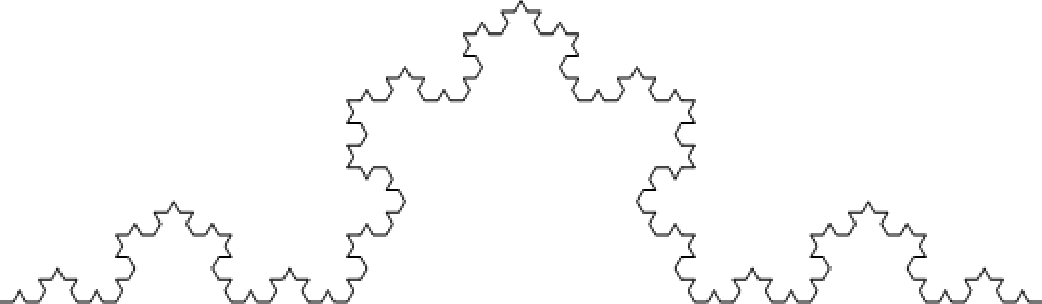
\includegraphics[width=1.0\textwidth]{koch_picture}
\caption{
Chiamato $K_0 \in \RR^2$ il segmento $[0,1]\times \{0\}$,
in figura è rappresentata
la quarta iterata $K_4 = T^4(K_0)$ della contrazione che definisce la curva di K{\"o}ch.
A pagina~\pageref{code:Koch} il codice per generare la figura in copertina.
\index{curva di K{\"o}ch}
}
\label{fig:koch}
\end{figure}

\begin{example}[curva di K{\"o}ch]
Sia $R_\theta\colon \RR^2 \to \RR^2$ la rotazione di $\RR^2$ con centro l'origine di $\theta$ radianti in senso antiorario.
Sia $\alpha = \pi/3$, $p=(1,0)$ e
siano $\phi_1, \phi_2, \phi_3, \phi_4 \colon \RR^2 \to \RR^2$
le funzioni definite da:
\begin{align*}
\phi_1(v) = \frac{v}{3}, \qquad
\phi_2(v) = R_{\alpha}\frac{v}{3} + \phi_1(p), \\
\phi_3(v) = R_{-\alpha}\frac{v}{3} + \phi_2(p), \qquad
\phi_4(v) = \frac{v}{3} + \phi_3(p).
\end{align*}
Allora esiste un unico insieme chiuso $K\subset \RR^2$ tale che
\[
  K = \phi_1(K) \cup \phi_2(K) \cup \phi_3(K) \cup \phi_4(K).
\]
L'insieme $K$ si chiama \myemph{curva di K{\"o}ch}. E' un frattale autosimile in quanto è composto da quattro copie riscalate di se stesso.
\end{example}


\section{Convergenza integrale}

Motivati da come viene definita la norma di un vettore
in $\RR^n$ risulta naturale
dare la seguente definizione di
\emph{norma euclidea} per una funzione $f\colon (a,b)\to \RR$:
\[
  \Abs{f}_2 = \sqrt{\int_a^b \abs{f(x)}^2\, dx}.
\]
Questa definizione ha senso, come integrale improprio, se la funzione $f$
è localmente Riemann-integrabile sull'intervallo $(a,b)$
(definizione~\ref{def:localmente_riemann}).
In tal
caso l'integrale esiste, ma potrebbe assumere il valore $+\infty$. Definiamo
allora
\[
\H(a,b) =
\{\text{$f$ localmente R.-integrabile su $(a,b)$}\colon \Abs{ f}_2< +\infty\}.
\]

Cercheremo ora di dimostrare che la norma che abbiamo introdotto
è effettivamente un norma (nel senso della definizione~\ref{def:norma})
che rende $\H(a,b)$ uno spazio vettoriale euclideo di dimensione infinita.

Innanzitutto è chiaro che qualunque sia $f$ si ha
$\Abs{ f}_2\ge 0$.
Inoltre è banale osservare che la norma è omogenea: se $t\in \RR$ si ha:
\[
  \Abs{t\cdot f}_2= \abs{t}\cdot \Abs{f}_2.
\]
Dunque se $f\in \H(a,b)$ anche $t f\in \H(a,b)$ per ogni $t \in \RR$.
Se $f,g\in \H(a,b)$ per la proprietà del parallelogramma~\eqref{eq:parallelogramma}
valida in $\RR$ si ha
\[
  (f(x) + g(x))^2 \le 2f^2(x) + 2 g^2(x)
\]
e dunque se $f,g \in \H(a,b)$ anche $f+g\in \H(a,b)$.
Dunque $\H(a,b)$ è uno spazio vettoriale.

Per $f,g\in \H(a,b)$ possiamo ora definire il prodotto scalare:
\begin{equation}\label{eq:854392}
  \langle f, g\rangle = \int_a^b f(x) \cdot g(x)\, dx.
\end{equation}
La disuguaglianza di
Young~\eqref{eq:Young} valida in $\RR$ ci dice che
\[
  \abs{f(x) \cdot g(x)} \le \frac{f^2(x)+g^2(x)}{2}
\]
e dunque garantisce che l'integrale~\eqref{eq:854392}
sia assolutamente convergente. Dunque se $f,g\in \H(a,b)$
il prodotto scalare $\langle f,g\rangle$ è ben definito ed
è un numero finito. A questo punto è facile verificare
che $\langle f,g\rangle$ è una forma bilineare simmetrica
non negativa. Dunque soddisfa tutte le proprietà formali
date nella definizione~\ref{def:prodotto_scalare} di prodotto scalare
salvo il fatto che non è garantito che $\langle f,f\rangle = 0$
implichi $f=0$. In effetti questa proprietà è falsa perché
se la funzione $f^2(x)$ ha integrale nullo non è detto che sia
identicamente nulla: l'integrale, infatti, non cambia
se la funzione viene modificata in un singolo punto.

Per ovviare a questo problema bisogna che identifichiamo due
funzioni $f,g\in \H(a,b)$ se $\Abs{f-g}_2=0$:
\[
  f \sim g  \iff \Abs{f-g}_2=0.
\]
Chiamiamo $H(a,b)$ il quoziente:
\[
  H(a,b) = \H(a,b)/\sim
\]
cioè lo spazio vettoriale delle funzioni in $\H(a,b)$ dove due funzioni
vengono identificate se la norma della differenza è nulla
(si vedano gli appunti di logica~\cite{appunti_logica}
per la definizione di insieme quoziente).

Lo spazio quoziente $H(a,b)$ risulta finalmente essere uno spazio
euclideo. Mantiene infatti la struttura vettoriale (in quanto l'insieme
$\{f\in \H(a,b)\colon \Abs{f}_2=0\}$ è uno spazio vettoriale)
e il prodotto scalare $\langle f,g\rangle$ (e di conseguenza la norma $\Abs{f}_2$)
è ben definito su $H(a,b)$ e oltre alle proprietà che già abbiamo dimostrato
possiamo ora affermare che $\langle f,f\rangle = \Abs{f}_2=0$ se e solo se $f=0$.

\begin{remark}
La notazione $H(a,b)$ che scegliamo di utilizzare per definire questo spazio
non è standard. La lettera $H$ rimanda ad Hilbert in quanto lo studio di questo
spazio in particolare ha spinto verso l'astrazione del concetto di spazio di Hilbert.
Quello che vedremo nel seguito è che questo spazio
non risulta essere completo e dunque in realtà non è uno spazio di Hilbert.
In effetti l'utilizzo degli integrali impropri è un tentativo, di
estendere l'integrale di Riemann in modo da rendere completo questo spazio.
Solo con la definizione di integrale di Lebesgue (1875--1941)
si è riusciti ad estendere l'integrale di Riemann
ad una classe più amplia di funzioni fino a completare lo spazio.
L'analogo dello spazio $H(a,b)$ definito tramite integrale di Lebesgue
viene
usualmente chiamato $L^2$. L'esponente $2$ è dovuto al fatto che
sarebbe possibile definire gli spazi $L^p$
in maniera analoga a quanto fatto nell'esempio~\ref{ex:norma_p}.
Si avrebbe ancora che solo per $p=2$ questi spazi normati sono euclidei,
cioè solo per $p=2$ la norma è indotta da un prodotto scalare.
Tutti gli spazi $L^p$ sono completi e dunque sono spazi di Banach.
Ma $L^2$ è anche uno spazio di Hilbert, in quanto è dotato di prodotto scalare.
Anzi potremmo dire che $L^2$ è lo spazio di Hilbert per antonomasia
e viene denotato anche con il nome $H^0$
(in questo caso l'esponente denota la derivabilità delle funzioni, come
in $C^0$).
\end{remark}

Gli elementi di $H(a,b)$ non sono funzioni, ma classi di equivalenza di funzioni.
Nel seguito, però, tratteremo $f\in H(a,b)$ come se fosse $f\in \H(a,b)$
facendo attenzione che le nostre affermazioni rimangano valide se al posto
di una funzione $f$ si prende una funzione a lei equivalente.
In particolare avrà senso considerare gli integrali di queste funzioni, perché il
valore dell'integrale non dipende dal rappresentante scelto, ma non avrà senso
considerare il valore che le funzioni assumono in un singolo punto, perché
questo dipende dal rappresentante.

\subsection{serie di Fourier}
\index{Fourier!serie di}%
\index{serie!di Fourier}%

Lo spazio $H(a,b)$ è uno spazio vettoriale reale su cui siamo riusciti a definire
un prodotto scalare e quindi una norma. Vorremmo trovare su $H(a,b)$ una base
ortonormale rispetto alla quale sia possibile scrivere le coordinate dei vettori
(cioè delle funzioni) di $H(a,b)$. Visto che $H(a,b)$ non ha dimensione finita
non potremo sperare di trovare una base con un numero finito di elementi.
Introduciamo quindi la seguente.

\begin{definition}[base hilbertiana]
\index{Hilbert!base di}
Sia $V$ uno spazio euclideo. Siano $e_k\in H(a,b)$ con $k\in \NN$. Diremo che
$e_k$ è un \myemph{sistema ortonormale} se $\langle e_k, e_j\rangle = 0$ quando
$k\neq j$ e $\langle e_k, e_k\rangle = 1$ per ogni $k\in \NN$.
Diremo che $e_k$ è una \myemph{base!hilbertiana} se è un sistema ortonormale
e inoltre per ogni $v\in V$
esistono $c_k\in \RR$ con $k\in\NN$ per cui si abbia
\begin{equation}\label{eq:49346}
  v = \sum_{k=0}^{+\infty} c_k e_k.
\end{equation}
\end{definition}

\begin{theorem}[disuguaglianza di Bessel]
Sia $e_0, e_1, e_2, \dots$ un sistema ortonormale in uno spazio euclideo $V$.
Per ogni $v\in V$ e per ogni $k\in \NN$ si ponga $c_k = \langle v,e_k\rangle$.
Allora vale la
\myemph{disuguaglianza!di Bessel}:
\index{Bessel!disuguaglianza di}
\begin{equation}\label{eq:disuguaglianza_Bessel}
\sum_{k=0}^{+\infty} c_k^2 \le \abs{v}^2.
\end{equation}

Inoltre possiamo affermare che il sistema ortonormale $e_0, e_1, e_2, \dots$
è una base hilbertiana se e solo se per ogni $v\in V$ vale l'uguaglianza:
\begin{equation}\label{eq:487562}
\sum_{k=0}^{+\infty} c_k^2 = \abs{v}^2.
\end{equation}
\end{theorem}
%
\begin{proof}
Dato $v\in V$ poniamo $c_k = \langle v,e_k\rangle$ e
\[
   v_N = \sum_{k=0}^N c_k e_k, \qquad w_N = v - v_N.
\]
Osserviamo che per ogni $n\in \NN$ si ha $\langle v_N,w_N\rangle=0$
($w_N$ è ortogonale a $v_N$)
in quanto se $n\le N$:
\[
  \langle w_N , e_n \rangle
  = \langle v, e_n\rangle - \sum_{k=0}^N c_k \langle e_k, e_n\rangle
  = \langle v,e_n\rangle - c_n = 0
\]
e quindi
\[
 \langle w_N, v_N \rangle = \sum_{k=0}^N c_k \langle w_N, e_k\rangle = 0.
\]
dunque possiamo concludere, grazie al teorema di Pitagora~\eqref{eq:Pitagora}
\begin{align*}
  \abs{v}^2
  &= \abs{v_N + w_N}^2
  = \abs{v_N}^2 + \abs{w_N}^2 \\
  &\ge \abs{v_N}^2 = \abs{\sum_{k=0}^N c_k e_k}^2
  = \sum_{k=0}^N c_k^2.
\end{align*}
Passando al limite per $N\to +\infty$ si ottiene la disuguaglianza
di Bessel.

Il sistema è hilbertiano, per definizione, se e solo se $v_N \to v$
ovvero se $w_N\to 0$.
Ma abbiamo visto che $\abs{w_N}^2 = \abs{v}^2 - \abs{v_N}^2$
dunque la condixione $\abs{w_N}^2\to 0$ è equivalente
all'uguaglianza di Bessel: $\abs{v_N}^2 \to \abs{v}^2$.
\end{proof}

Il nostro obiettivo è ora quello di produrre una base hilbertiana di $H(-\pi,\pi)$.
Consideriamo le seguenti funzioni trigonometriche:
\begin{equation}\label{eq:54741346}
\begin{aligned}
  e_0 (x) &= \frac{1}{\sqrt{2\pi}} \\
  e_{2k+1}(x) &= \frac{\sin(kx)}{\sqrt{\pi}} \qquad k=0,1,\dots\\
  e_{2k}(x) &= \frac{\cos(kx)}{\sqrt{\pi}} \qquad k=1,2,\dots
\end{aligned}
\end{equation}
Ovviamente
\[
  \Abs{e_0}_2=\sqrt{\int_{-\pi}^{\pi} \enclose{\frac{1}{\sqrt{2\pi}}}\, dx} = 1
\]
ma è anche facile verificare che
\[
  \int_{-\pi}^{\pi} \cos^2 (kx)\, dx
  = \frac{1}{k}\int_{-k\pi}^{k\pi} \cos^2 y\, dy
  = \int_{-\pi}^{\pi} \cos^2 y\, dy = \pi
\]
da cui si ottiene $\Abs{e_{2k}}_2 = 1$.
Visto che la funzione $\sin$ è la traslata di $\cos$ si
ottiene analogamente che $\Abs{e_{2k+1}}_2=1$.
Dunque i vettori $e_0,e_1,\dots$ sono tutti di modulo unitario.
Utilizzando la formula di Eulero
si può trovare la formula di Werner:
\index{Werner!formula di}%
\index{formula!di Werner}%
\begin{align*}
 \sin(mx)\cos(nx)
 &= \frac{e^{inx}-e^{-inx}}{2}\cdot \frac{e^{imx}-e^{-imn}}{2i}\\
 &= \frac{e^{i(m+n)x}}{4i} + \frac{e^{-i(m+n)x}}{4i} + \frac{e^{i(m-n)x}}{4i} - \frac{e^{-i(m-n)x}}{4i}\\
 &= \frac{\sin\enclose{(m+n)x}}{2} + \frac{\sin\enclose{(m-n)x}}{2}
\end{align*}
da cui se $m\neq n$:
\begin{align*}
 \int_{-\pi}^{\pi} \sin(mx)\cos(nx)\, dx &=
 -\frac 1 {2(m+n)} \Enclose{\cos\enclose{(m+n)x}}_{-\pi}^{\pi} \\
  &\quad - \frac{1}{2(m-n)}\Enclose{\cos\enclose{(m-n)x}}_{-\pi}^{\pi} = 0
\end{align*}
e se $m=n$ si arriva comunque allo stesso risultato.
Questo significa che $\langle e_{2n},e_{2m+1}\rangle = 1$.
Discorso analogo si può fare per le funzioni $\sin(mx)\sin(nx)$ e $\cos(mx)\cos(nx)$
trovando, anche in quei casi, che tali prodotti hanno integrale nullo
nell'intervallo $[-\pi,\pi]$.
Per nostra memoria le formule di Werner che si trovano
in questi ultimi casi sono:
\index{Werner!formula di}%
\index{formula!di Werner}%
\begin{align*}
  \cos(mx) \cos(nx) &=  \frac{\cos((m+n)x)}{2} + \frac{\cos((m-n)x)}{2}\\
  \sin(mx) \sin(nx) &=  \frac{\cos((m-n)x)}{2} - \frac{\cos((m+n)x)}{2}.
\end{align*}

Risulta dunque che le funzioni $e_0,e_1,e_2,\dots$ definite da~\eqref{eq:54741346}
formano un sistema ortonormale in $H(-\pi,\pi)$
in quanto si ha:
\[
  \langle e_n, e_m \rangle =
  \begin{cases} 1 &\text{se $m=n$}\\
  0 & \text{altrimenti}.
  \end{cases}
\]
Di conseguenza le funzioni $e_0,e_1,e_2, \dots$ sono tra loro indipendenti
in $H(-\pi,\pi)$ in quanto se una loro combinazione lineare è nulla:
\[
  \sum_{k=0}^n \lambda_k e_k = 0
\]
allora, facendone il prodotto scalare con $e_j$ si ottiene:
\[
  0 = \langle \sum_{k=0}^n \lambda_k e_k , e_j\rangle
  = \sum_{k=0}^n \lambda_k \langle e_k, e_j\rangle
  = \lambda_j
\]
e dunque tutti i coefficienti $\lambda_j$ sono nulli.
Possiamo in particolare dedurre che $H(-\pi,\pi)$ ha dimensione
infinita.

\begin{definition}[polinomi trigonometrici]
Una funzione $f$ si dice essere un \myemph{polinomio trigonometrico}
se esiste un polinomio in due variabili $P(X,Y)$ tale che
\[
  f(x) = P(\cos x, \sin x).
\]
\end{definition}

Possiamo verificare che $f$ è un polinomio trigonometrico se e solo se
è possibile scrivere $f$ come combinazione lineare finita delle funzioni $e_k$
appena introdotte,
cioè se esistono $c_0, c_1, \dots, c_n\in \RR$ tali che
\[
  f = \sum_{k=0} c_k e_k.
\]
Basta infatti ricondurre le funzioni trigonometriche all'esponenziale complesso,
tramite la formula di Eulero:
\begin{align*}
   \cos(nx) + i \sin(nx)
   &= e^{inx} = (e^{in})^k
   = \enclose{\cos x + i \sin x}^n\\
   &= \sum_{k=0}^n {n \choose k} i^k \enclose{\sin x}^k \enclose{\cos x}^{n-k}
\end{align*}
da cui, prendendo parte reale, e parte immaginaria si
riesce ad esprimere $\cos(nx)$ e $\sin(nx)$ come polinomio in $\sin x$ e $\cos x$.
Più precisamente per il coseno
si ottengono solo i termini con $k$ pari:
\begin{align*}
\cos(nx) &= \sum_{k=0}^{\floor{\frac n 2}} {n \choose 2k} (-1)^k \enclose{\sin x}^{2k} \enclose{\cos x}^{n-2k}\\
&= \sum_{k=0}^{\floor{\frac n 2}}{n \choose 2k} \enclose{\cos^2 x -1}^k \enclose{\cos x}^{n-2k}
\end{align*}
ovvero
\[
  \cos(nx) = T_n(\cos x)
\]
dove
\[
  T_n(x) = \sum_{k=0}^{\floor{\frac n 2}}{n \choose 2k} \enclose{x^2 -1}^k x^{n-2k}
\]
si chiama \emph{polinomio di Chebyshev di prima specie}.
\index{polinomio!di Chebyshev}%
\index{Chebyshev!polinomio di}%
Questo significa che ognuna delle funzioni $e_k$ che abbiamo introdotto
in~\eqref{eq:54741346} è un polinomio trigonometrico e quindi ogni
combinazione finita di tali funzioni è ancora un polinomio trigonometrico.

Viceversa per verificare che ogni polinomio trigonometrico può essere rappresentato
come combinazione lineare finita degli elementi $e_k$
possiamo osservare che se $f(x) = P(\cos x,\sin x)$ è un polinomio trigonometrico
allora usando le formule di Eulero si può scrivere $f(x) = Q(e^{ix}, e^{-ix})$
dove $Q$ è un polinomio a coefficienti complessi. Ma osservando che
\[
  \enclose{e^{ix}}^n = e^{inx}
\]
si ottiene che $f(x)$ può essere scritta come combinazione lineare complessa
delle funzioni $e^{ikx}$ e $e^{-ikx}$. Utilizzando nuovamente le fomule di
Eulero si deduce che $f(x)$ può essere scritta come combinazione lineare
complessa delle funzioni $\cos(ikx)$ e $\sin(ikx)$:
\[
  f(x) = \sum_{k=0}^n \enclose{z_k \cos(ikx) + w_k \sin(ikx)}.
\]
Ma visto che sappiamo che $f(x)$ è una funzione reale, la somma delle parti
immaginarie di questa combinazione lineare è nulla e dunque abbiamo ottenuto
che $f(x)$ è combinazione lineare a coefficienti reali
delle funzioni $e_n$.

\begin{definition}[serie di Fourier]
Se $f\in \H(a,b)$ i coefficienti $c_k = \langle f, e_k\rangle$
si chiamano \myemph{coefficienti di Fourier} di $f$
e la serie
\[
  \sum_{k=0}^{+\infty} c_k e_k
\]
si chiama \myemph{serie di Fourier} di $f$. Il polinomio
trigonometrico
\[
  f_N = \sum_{k=0}^{N} c_k e_k
\]
è si chiama \myemph{sviluppo di Fourier} di ordine $N$ per $f$.
\end{definition}

\begin{figure}
\begin{center}
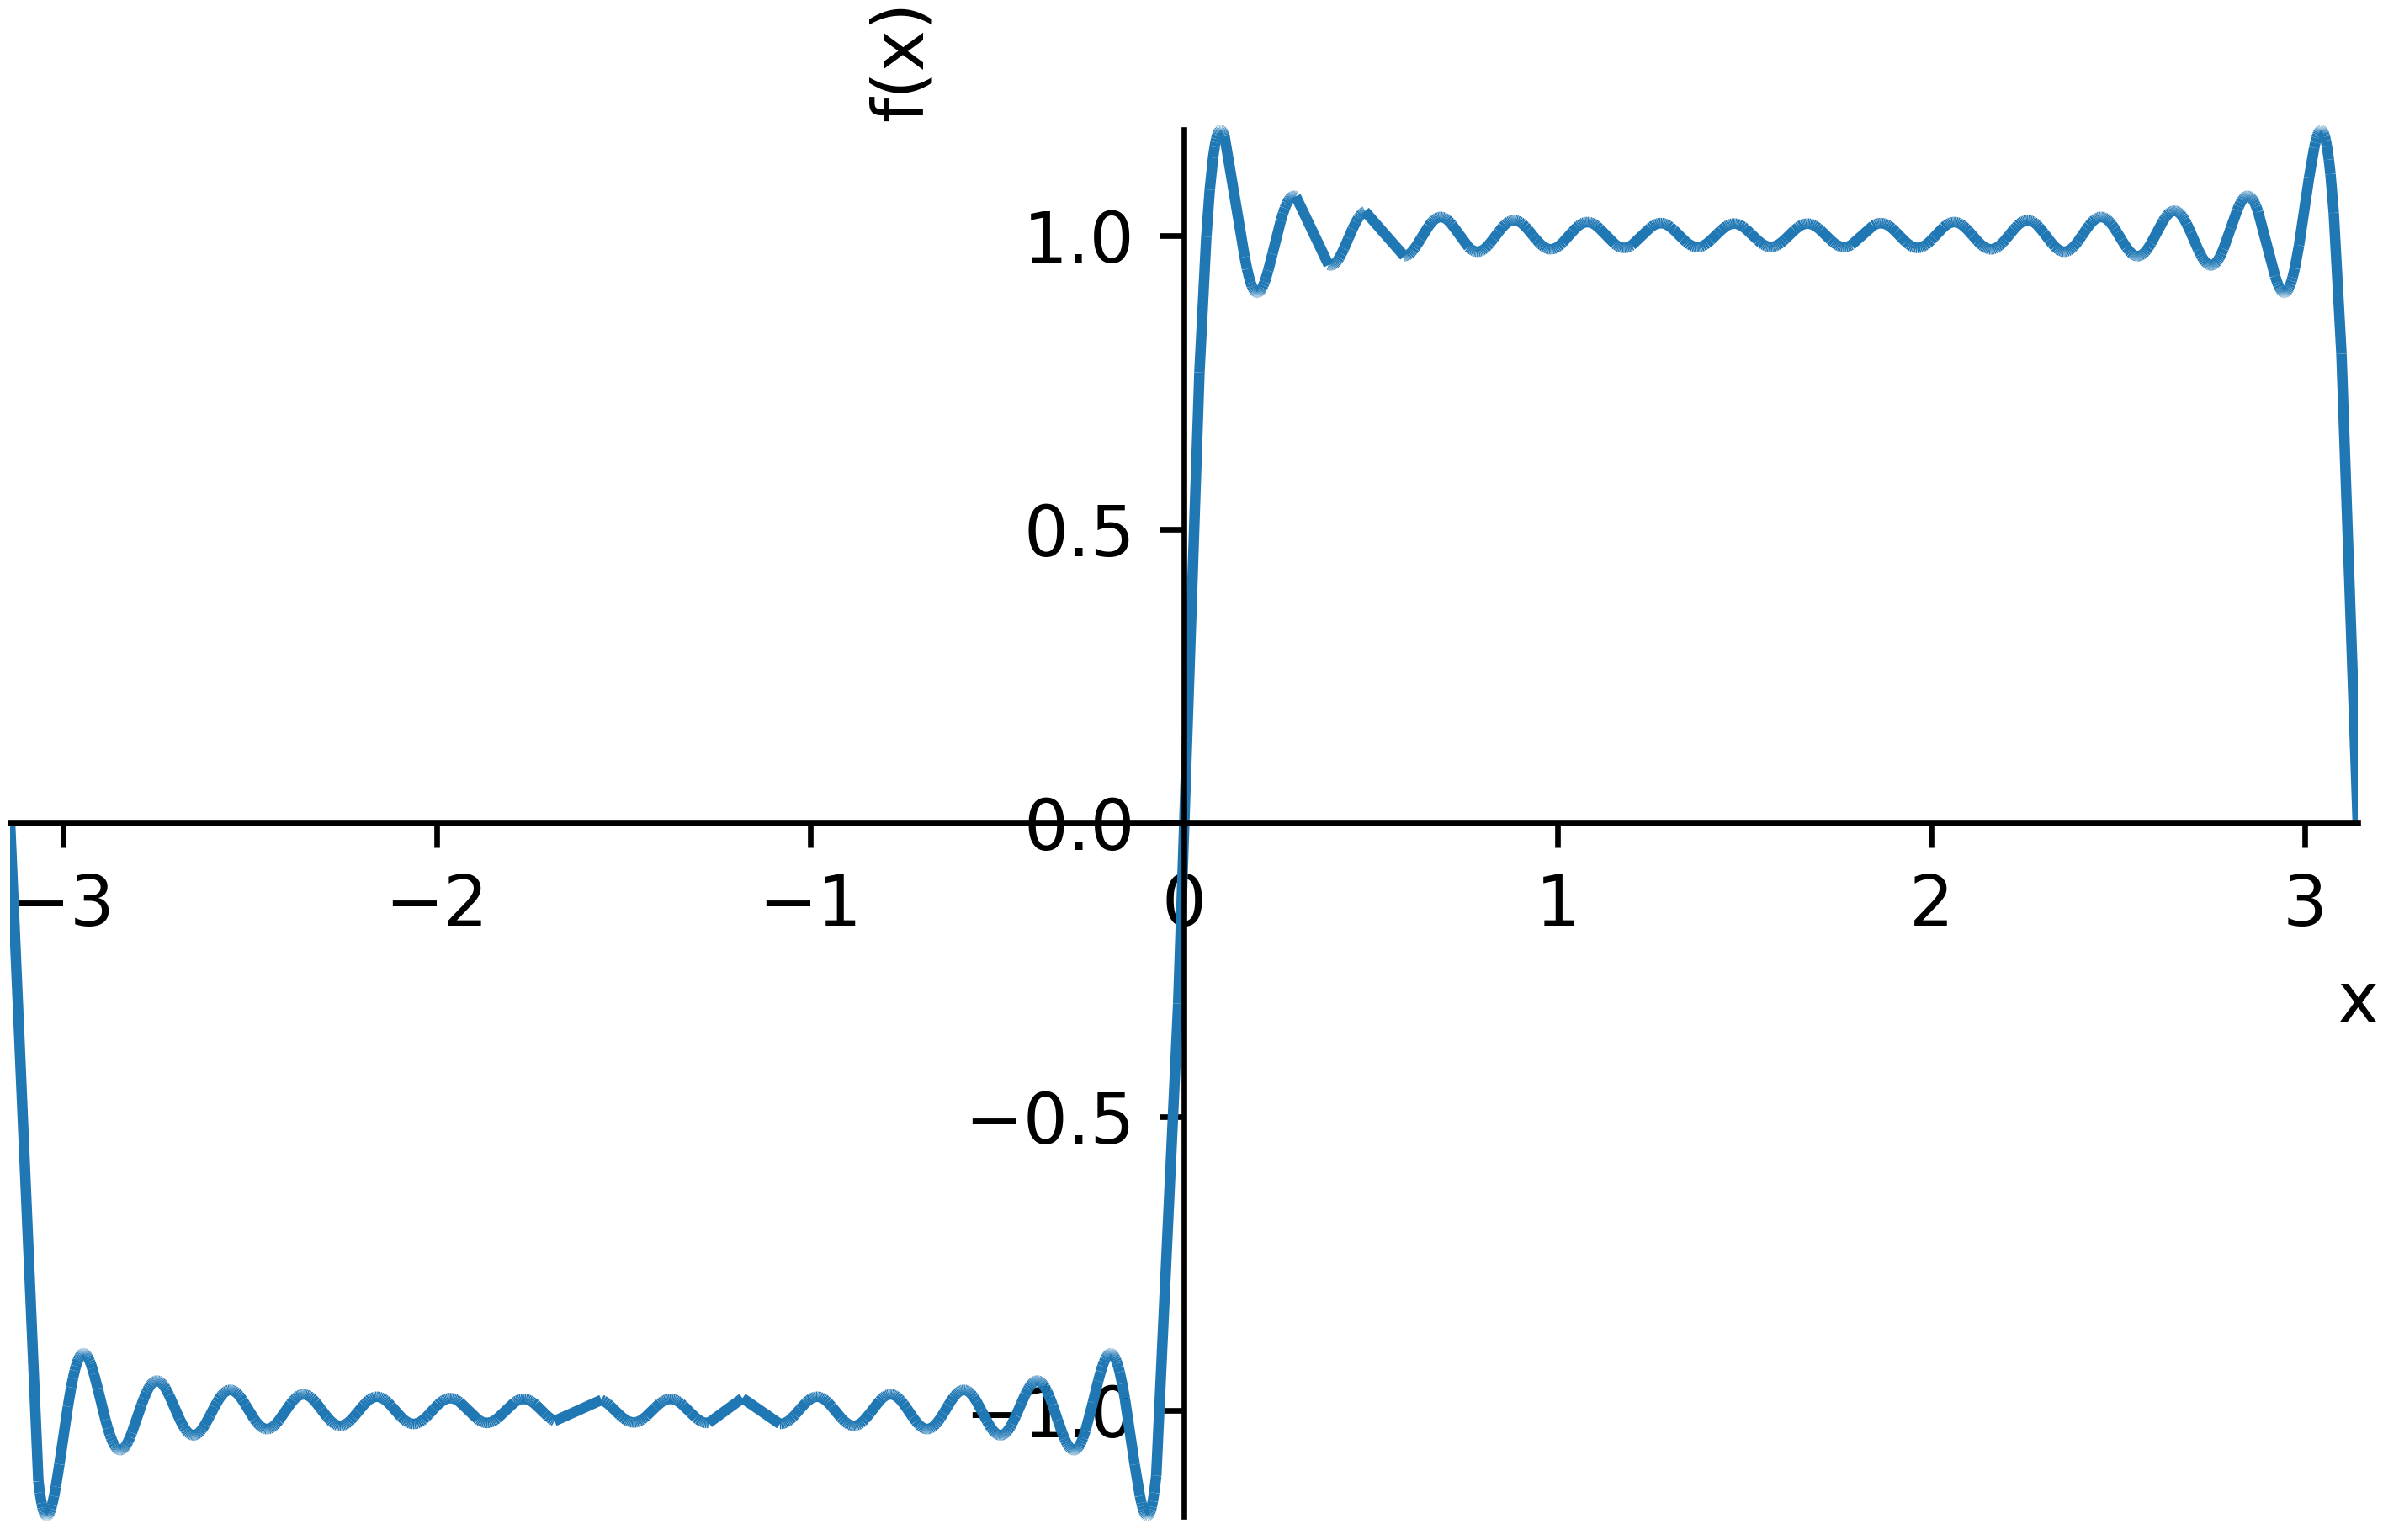
\includegraphics[height=5cm]{fourier.png}
\end{center}
\captionsetup{singlelinecheck=off}
\caption{Lo sviluppo di Fourier della funzione
che vale $1$ su $[0,\pi]$ e $-1$ su $[-\pi,0]$:
$
f_{61}(x)=
\frac{4\sin(x)}{\pi} + \frac{4\sin(3x)}{3\pi} + \frac{4\sin(5x)}{5\pi} + \frac{4\sin(7x)}{7\pi} + \frac{4\sin(9x)}{9\pi} + \frac{4\sin(11x)}{11\pi} + \frac{4\sin(13x)}{13\pi} + \frac{4\sin(15x)}{15\pi} + \frac{4\sin(17x)}{17\pi} + \frac{4\sin(19x)}{19\pi} + \frac{4\sin(21x)}{21\pi} + \frac{4\sin(23x)}{23\pi} + \frac{4\sin(25x)}{25\pi} + \frac{4\sin(27x)}{27\pi} + \frac{4\sin(29x)}{29\pi} + \frac{4\sin(31x)}{31\pi}
$.
Il codice python per generare il grafico
a pagina~\pageref{code:Fourier}
}
\label{fig:fourier}
\end{figure}

Risulta naturale chiedersi se quella che abbiamo introdotto è una
\emph{base hilbertiana} perché solo in tal caso gli sviluppi di Fourier
approssimano la funzione.
Per ottenere questo risultato dobbiamo assumere la validità del seguente
teorema, che sarebbe ora troppo lungo dimostrare.

\begin{theorem}[densità dei polinomi trigonometrici]
Per ogni funzione continua $f\in C^0([a,b])$
esiste una successione $g_k\in \H(a,b)$ di polinomi trigonometrici
(cioè combinazioni lineari finite del sistema $\{e_k\}$)
tale che $g_k$ converge uniformemente a $f$.

Detto in altri termini: l'insieme dei polinomi trigonometrici
è denso nello spazio $C^0([a,b])$ rispetto alla norma uniforme.
\end{theorem}

Osserviamo che la convergenza uniforme è più forte della convergenza
in $H(a,b)$ in quanto si ha, banalmente:
\[
  \Abs{f}_2^2 = \int_a^b f(x)^2\, dx
  \le \int_a^b \Abs{f}_\infty^2\, dx
  = (b-a) \Abs{f}_\infty^2.
\]
Dunque il teorema precedente garantisce che ogni funzione continua
in $\H(a,b)$ può essere approssimata, rispetto alla norma $\Abs{\cdot}_2$,
tramite polinomi trigonometrici. Il teorema seguente ci permette
di estendere questa proprietà a tutte le funzioni di $\H/(a,b)$.

\begin{theorem}[densità delle funzioni continue]
Data una qualunque $f\in H(a, b)$ per ogni $\eps>0$
esiste una funzione continua $g\colon [a,b]\to \RR$
tale che $\Abs{f-g}_2<\eps$.

Detto in altri termini: $C^0([a,b])$ è un sottospazio denso in $H(a,b)$
cioè un insieme la cui chiusura (nella topologia di $H(a,b)$) è tutto $H(a,b)$.
\end{theorem}
%
\begin{proof}
Se $f\in H(a,b)$ si ha,
per la disuguaglianza di Cauchy-Schwarz:
\[
  \int_a^b \abs{f(x)}\, dx
  \le \Abs{1}_2 \cdot \Abs{f}_2 = \sqrt{b-a}\cdot \Abs{f}_2 < +\infty.
\]
Dunque la funzione $f$ è assolutamente integrabile su $(a,b)$.
Se $f$ è limitata su $(a,b)$ possiamo pensare che $f$ sia definita su $[a,b]$
e l'integrale è un usuale integrale di Riemann (non improprio).
Per le condizioni di integrabilità sappiamo che per ogni $\eps>0$ è possibile
trovare una suddivisione $a=x_0 < x_1 < \dots < x_n =b$ su cui l'integrale
di $f$ differisce dagli integrali superiore e inferiore per meno di $\eps$.
Possiamo prendere come funzione $g$ una interpolazione lineare
cioè una funzione tale che si abbia $g(x_k) = f(x_k)$ sui punti della suddivisione
e che risulti lineare su ogni intervallino $[x_k,x_{k+1}]$. La funzione
$g$ così definita è compresa, su ogni intervallino, tra l'$\inf$ e il $\sup$
di $f$ e dunque si avrà:
\[
 \int_a^b \abs{f(x)-g(x)}\, dx < \eps.
\]
Visto però che $f$ è limitata sappiamo esistere $M>0$ per cui $\Abs{f}_\infty\le M$
e di conseguenza $\Abs{g}_\infty\le M$ e quindi $\Abs{f-g}_2\le 2M$.
Ma allora
\[
  \Abs{f-g}_2^2 = \int_a^b \abs{f(x)-g(x)}^2\, dx
  \le \int_a^b \Abs{f-g}_\infty \cdot \abs{f(x)-g(x)}\, dx
  \le 2M \eps.
\]
Abbiamo quindi mostrato che una funzione limitata e integrabile può essere
approssimata con funzioni continue.

Se la funzione è integrabile in senso improprio su $(a,b)$ ma non è limitata, per
definizione di integrale improprio per ogni $\eps>0$ possiamo trovare un intervallo
$[\alpha,\beta]\subset (a,b)$
per $f$ risulta limitata su $[\alpha,\beta$] e
l'integrale di $f$ su $(a,b)$ differisce dall'integrale di $f$ su $[\alpha,\beta]$
per meno di $\eps$. Ci possiamo quindi ricondurre al passo precedente
per trovare una funzione $g$ che approssima bene $f$ sull'intervallo $[\alpha,\beta]$.
Estendendo $g$ in modo costante su $(a,b)\setminus[\alpha,\beta]$ si troverà
una funzione che approssima bene $f$ su tutto $(a,b)$.
\end{proof}

Grazie ai due teoremi precedenti sappiamo che ogni $f\in \H(a,b)$ può essere
approssimata da polinomi trigonometrici $g_N\to f$
cioè da funzioni della forma:
\[
  g_N = \sum_{k=0}^{N} a_{k,N} e_k.
\]
Stiamo qui assumendo che il polinomio trigonometrico $g_N$ abbia ordine non superiore
ad $N$, ma questo si può sempre assumere, scartando
o ripetendo i termini della successione.

Se ora consideriamo gli sviluppi di Fourier:
\[
  f_N = \sum_{k=0}^N c_k e_k, \qquad c_k = \langle f,e_k\rangle
\]
ci ricordiamo che per ogni $k\le N$ risulta
\[
   \langle f-f_N, e_k \rangle
   = \sum{k=0}^N \enclose{\langle f,e_k\rangle - c_k} = 0
\]
e quindi
\[
  \langle f-f_N , g_N -f_N\rangle
  = \sum_{k=0}^N \langle f-f_N, (a_{k,N}-c_k) e_k \rangle
  = 0.
\]
Dunque, applicando il teorema di Pitagora,
\[
  \Abs{f-f_N}_2^2 = \Abs{f-g_N}_2^2 - \Abs{f_N-g_N}_2^2
  \le \Abs{f-g_N}_2^2 \to 0.
\]
Questo significa, dunque, che il sistema ortonormale che abbiamo introdotto
è una base hilbertiana e quindi che ogni funzione $f\in \H(a,b)$ si approssima
rispetto alla norma $\Abs{\cdot }_2$ con gli sviluppi di Fourier.

Ricordiamo che se $\Abs{f_N-f}_2 \to 0$ non è detto che si abbia la convergenza
puntuale $f_N(x)\to f(x)$ per ogni $x\in (a,b)$ in quanto il limite è unico
in $H(a,b)$ ma non in $\H(a,b)$ e dunque è possibile (e in effetti può succedere)
che il limite puntuale degli sviluppi di Fourier differisca, in alcuni punti,
dalla funzione che si sta approssimando.

Purtroppo lo spazio $H(a,b)$ non risulta essere
completo, come si può vedere nel seguente esempio.

\begin{example}[razionali ingrassati]
\label{ex:incompletezza_di_H}
Vogliamo mostrare che lo spazio $H(0,1)$ non è completo.
Sappiamo che l'insieme $[0,1]\cap \QQ$ è numerabile, quindi esiste una
successione $q_k$ che elenca tutti i numeri razionali nell'intervallo $[0,1]$.
Poniamo inoltre $r_k = \frac{1}{4\cdot 2^k}$ e consideriamo gli intervalli
$I_k = [q_k-r_k,q_k+r_k]$.
Prendiamo la successione di funzioni $f_n\colon [0,1]\to \RR$
definita da
\[
  f_n(x) =
  \begin{cases}
  1 &\text{se } x\in\displaystyle\bigcup_{k=1}^{n} I_k\\
  0 & \text{altrimenti}
  \end{cases}
\]
A differenza di quanto uno potrebbe pensare, queste funzioni $f_n$ non diventano
mai identicamente uguali ad $1$. Anzi, si può osservare che
\[
  \int_0^1 f_n(x)\, dx
  \le \sum_{k=1}^n \int_{q_k-r_k}^{q_k+r_k} 1\, dx
  = \sum_{k=1}^n \frac{1}{2\cdot 2^k}
  \le \frac{1}{2}\sum_{k=1}^{+\infty}\frac{1}{2^k} = \frac 1 2.
\]

Vogliamo ora mostrare che $f_k$ è una successione di Cauchy in $H(0,1)$ e
che però non converge in $H(0,1)$.

Per verificare che $f_n$ è una successione di Cauchy possiamo semplicemente
osservare che se $n\ge m$ risulta che $f_n$ e $f_m$ differiscono solamente
sugli intervalli $I_k$ con $k$ compreso tra $m$ ed $n$. Dunque:
\[
  \int_0^1 \abs{f_n - f_m}
  \le \sum_{k=m}^{+\infty} \int_{q_k-r_k}^{q_k+r_k} 1\,dx
  = \sum_{k=m}^{+\infty}\frac{1}{2\cdot 2^k} = \frac{1}{2^m}.
\]
Visto che $f_n$ e $f_m$ assumono solamente i valori $0$ e $1$ anche $\abs{f_n-f_m}$
assume solamente i valori $0$ e $1$ quindi $\abs{f_n-f_m}^2=\abs{f_n-f_m}$.
Abbiamo quindi verificato che per $n\ge m$ si ha:
\[
  \Abs{ f_n - f_m}_2 \le \sqrt{\frac{1}{2^m}}.
\]
E' dunque chiaro che comunque sia scelto $\eps>0$ possiamo scegliere $N$
tale che $1/2^N \le \eps^2$ da cui si ottiene che se $n,m\ge N$
allora $\Abs{ f_n-f_m}_2 \le \eps$. Cioè: $f_n$ è una successione di Cauchy.

Supponiamo ora, per assurdo, che esista $f\in H(0,1)$
tale che $\Abs{ f_n-f}_2 \to 0$.
Innanzitutto visto che ogni $f_k\le 1$ possiamo supporre che sia anche $f\le 1$
perché altrimenti potremmo prendere $g(x) = \min\{f(x),1\}$ e avremmo
chiaramente $\Abs{f_n - g}_2 \le \Abs{f_n -f}_2 \to 0$. In pratica stiamo dicendo
che modificando la funzione $f$ senza cambiarne l'integrale possiamo suppore
che $f(x)\le 1$ per ogni $x\in[0,1]$.

Fissato un intervallo $I_n$, per $k\to +\infty$ si ha:
\[
  0\le \int_{q_n-r_n}^{q_n+r_n}\abs{f_k(x)-f(x)}^2\, dx
  \le \int_0^1 \abs{f_k(x)-f(x)}^2\, dx = \Abs{ f_k -f}_2^2 \to 0.
\]
Ma ora se $k\ge n$ risulta che $f_k=1$ su $I_n$ e quindi il valore dell'integrale
precedente non dipende da $k$ e dovrà quindi essere identicamente nullo:
\[
  \int_{q_n-r_n}^{q_n+r_n} f(x) - 1 \, dx = 0
\]
e quindi possiamo affermare che $\sup f(I_n) = 1$ in quanto se fosse
$\sup f(I_n) = \lambda < 1$
l'integrale di $f(x)-1$ sarebbe negativo
sull'intervallo $I_n$.

Vogliamo ora dimostrare che su ogni intervallo $[a,b]\subset[0,1]$ si ha
$\sup f([a,b])=1$. Prendiamo $N$ abbastanza grande in modo che $r_N < (b-a)/3$.
Allora l'intervallo $[a+r_n, b-r_n]$ ha ampiezza $r_n$ e contiene infiniti
numeri razionali. Esistono quindi infiniti indici $n$ per cui $q_n$ sta in tale
intervallo. Tra questi infiniti certamente ce n'è uno con indice $n\ge N$
(perché i $q_n$ con $n< N$ sono in numero finito). Ma se $q_n \in [a+r_n,b-r_n]$
allora $I_n\subset[a,b]$ e quindi $\sup f([a,b])\ge \sup f(I_n) = 1$.

Questo significa che per ogni suddivisione di Riemann dell'intervallo $[0,1]$
risulta che il $\sup$ di $f$ sugli intervallini della suddivisione è $1$ e quindi
l'integrale superiore di $f$ è anch'esso $1$. Dunque, essendo $f$ integrabile,
\[
  \int_a^b f(x) = 1.
\]

Vogliamo ora concludere che questo è in contraddizione con la disuguaglianza
\[
  \int_a^b f_n(x) \le \frac 1 2
\]
che abbiamo osservato all'inizio.
Si ha infatti per la disuguaglianza di Cauchy-Schwarz
\begin{align*}
  \int_0^1 \abs{f(x)-f_n(x)}\, dx
  \le \Abs{f-f_n}_2\cdot \Abs{1}_2  \to 0
\end{align*}
e quindi, per il criterio di convergenza assoluta,
\[
  \int_0^1 (f(x) - f_n(x))\, dx \to 0.
\]
Ma abbiamo visto che
\[
  \int_0^1 (f(x) - f_n(x))\, dx
  = \int_0^1 f(x)\, dx - \int_0^1 f_n(x)\, dx
  \ge 1 - \frac 1 2 = \frac 1 2
\]
ottenendo quindi un assurdo.
\end{example}

Il fatto di avere trovato una base hilbertiana di $H(a,b)$ ci permette di
dire che ogni funzione in $H(a,b)$ può essere rappresentata dalle sue
coordinate $c_k$ in modo che valga l'uguaglianza di Bessel:
\[
  \Abs{f}_2 = \sqrt{\sum_{k=0}^{+\infty} c_k^2}.
\]
Abbiamo in effetti definito una corrispondenza:
\[
  \phi \colon H(a,b) \to \ell^2,
  \qquad
  \ell^2=\{c\in \NN^\RR \colon \sum_{k=0}^{+\infty} c_k^2<+\infty\}
\]
definita da
\[
  c_k = \phi(f) = \langle f, e_k\rangle.
\]
Chiaramente tale $\phi$ è lineare. Visto che $e_k$ è una base hilbertiana
è facile verificare che $\phi$ è anche iniettivo. Se su $\ell^2$
definiamo il prodotto scalare e la norma corrispondente:
\[
  \langle x,y\rangle = \sum_{k=0}^{+\infty} x_k y_k, \qquad
  \abs{x}_2 = \sqrt{\sum_{k=0}^{+\infty}} x_k^2
\]
l'uguaglianza di Bessel ci dice che $\phi$ mantiene la norma e quindi
la struttura di spazio euclideo. Si potrebbe dimostrare che $\ell^2$
è completo e questo significa che $\phi$ non è suriettiva in quanto
la successione $f_n$
considerata nell'esempio~\ref{ex:incompletezza_di_H}
è di Cauchy in $H(a,b)$, dunque $\phi(f_n)$ è di Cauchy in $\ell^2$
e dunque converge in $\ell^2$. Il limite $c$ della successione $\phi(f_n)$
rappresenta una successione di coefficienti di Fourier che non possono
essere ottenuti da nessuna funzione $f\in H(a,b)$.
